\chapter{Scientific Computing: a story}
\label{chapter:context}
    %% TODO Historique : https://fr.wikipedia.org/wiki/Superordinateur#Historique_des_records

    \section{First computers, from carbon to silicon}%
    \label{sec:first_computers}

        % TODO talk about the human computers, followed by the first (machine) computer created by Cray and IBM, also
        % Von Neuman, analog computers, etc.
        Science has always been tightly associated to computations, hence this is no surprise that the first computers
        were not machines, but humans. Already in the second century AD, Ptolemy, a scientist living in Alexandria,
        wrote the Almagest. This book aggregated the state of the art in mathematics and astronomy and remained a
        reference for centuries. It contained several tables that were computed by the scientist, including a
        trigonometric table (called \emph{table of chords}).

        In 1757, three French astronomers, Clairaut, Lalande and Lepaute, started working on the prediction of the next
        appearances of Halley's comet~\cite[Chapter~1]{human_computers}. Using the recent theories of Newton, they had
        to numerically solve the three-body problem: they computed the orbits of Saturn and Jupiter around the Sun,
        taking into account the attraction force between the two planets. They carried this computation by splitting the
        orbits in tiny steps, computing the new planet locations for each step. They used these sequences of coordinates
        to compute the orbit of Halley's comet around the Sun, by taking into account the effect of the two giant
        planets on the comet and neglecting the effect of the comet itself on the three bodies. They were succesful in
        predicting the next appearance of the comet in the beginning of 1759, making an error of only one month. Their
        work constitutes one of the first recorded division of labor applied to computations, Lalande and Lepaute
        computed the orbits of the two giant planets while Clairaut computed the orbit of the comet.

        Gaspard de Prony, a French civil engineer, went a step further in this endeavor of organized
        computation~\cite[Chapter~2]{human_computers}. In 1791, he was named director of the \emph{Bureau du Cadastre}.
        At the time, the French revolutionary government was preparing reforms for their outdated system of weights and
        measures, which will eventually result in the creation of the metric system. The reforms proposed to measure
        angles in grades instead of degrees, dividing a right angle into 100 grades instead of 90 degrees. Prony was
        tasked to prepare trigonometric tables for this decimal grade system. He organized his staff in a hierarchy of
        three levels:
        \begin{itemize}
            \item The first class of workers, a handful of renowed scientists like Carnot or Legendre, oversaw the
                operations. They had to research the appropriate formulas for computing approximations of trigonometric
                functions with basic arithmetical operations.
            \item The second class, subsequently named \emph{planning commitee}, was a team of eight experienced
                computers. Their task consisted in translating the trigonometric equations produced by the first class
                into a sequence of additions and substractions. They prepared worksheets where all the basic operations
                were written with a blank space for the result.
            \item The third class consisted in nearly ninety computers. Many of them were former servants or wig makers
                that lost their jobs with the Revolution, they did not know any mathematics besides the addition and
                substraction. Their job was to compute the results to fill the blank spaces left by the second class of
                workers.
        \end{itemize}

        The idea of constructing a machine capable of doing computations is not recent. Already in 1642, Blaise Pascal,
        a French mathematician, invented and built a mechanical calculator that could perform the four arithmetical
        operations. The calculator was not commercialy viable at the time, so only twenty machines were built. Much
        later, in the first half of the nineteenth century, Charles Babbage~\cite[Chapters~2-3]{human_computers}, an
        English mathematician, invented two very innovative machines. The difference engine, for computing tables of
        polynomial functions, and the analytical engine, a general purpose computer that would subsequently be qualified
        as \emph{Turing-complete}. Unfortunately, due to a lack of funding, he was never able to build his inventions.
        In the same period, a French inventor named Thomas de Colmar designed and manufactured a digital
        mechanical calculator, called arithmometer. Capable of doing the four arithmetical operations, it was the first
        machine of its kind to be reliable enough for a practical use.  Similarly, Herman Hollerith, an American
        inventor, created the tabulating machine. Initialy built to process the 1890 US Census data, it worked by
        reading and summarizing information stored in punched cards. It decreased considerably the duration and cost of
        the whole census organization. These two last inventions~\cite[Chapter~6]{human_computers} were commercial
        successes and started an era of mechanical computations that lasted until the second half of the twentieth
        century.

        Gradually, computing became more and more important and recognized as a discipline. The apparition of modern
        statistics, mainly due to the work of Francis Galton and Karl Pearson in the early twentieth century, led to a
        growing need for computation power. The First World War itself was an important catalyzer, as the American,
        French and English governments hired entire computing laboratories to create ballistic
        tables~\cite[Chapter~10]{human_computers}. By the time, electromechanical computers were used everywhere, for
        their efficiency and reliability largely superior to human computers. There was still an important need for
        human labor, not only for operating these machines, but some complex operations were still carried by hand.

        The first working general purpose programmable computer, named \emph{Z3}, was designed and built more than two
        decades later in Germany by Konrad Zuse~\cite{sep-computing-history}. Completed in 1941, It was an
        electromechanical machine, using both (mechanical) relays and (electronic) vacuum tubes. Its programs, written
        on external tapes, could use loops but not conditional branches. In 1944, the British government built the first
        fully electronic computer, named \emph{Colossus}. Made of vacuum tubes, its primary function was to break the
        German ciphers during the war. Later, in 1945, the first US electronic computer was unveiled, called
        \emph{ENIAC}. Both the Colossus and ENIAC computers were programmed by plugboards and switches, instead of
        reading from a tape like the Z3. Interestingly, the Z3 and Colossus machines used binary arithmetic while the
        ENIAC used decimal representation.

        An important breakthrough came with the notion of stored-program computer, \ie the idea of storing the program
        instructions in memory. Although the original ideas can be traced to Turing himself and his 1936 article, the
        real implementation in electronical computers came several years later. The first stored-program computer was
        the \emph{Manchester Baby}, built at the University of Manchester in 1948~\cite{sep-computing-history}.
        Similarly, the successor of the ENIAC, called \emph{EDVAC} was also a stored-program computer. Yet, at the time,
        computers were still using vacuum tubes. Although this was a great reliability improvement to the mechanical
        parts used before, the vacuum tubes had a very large electricity consumption which started to become problematic
        (the ENIAC consummed \NSI{150}{\kilo\watt}, the EDVAC \NSI{56}{\kilo\watt}). They also required a large number of
        human operators for their daily usage.

        The invention of the transistor in 1947 by three Bell Labs physicists had a huge impact on the whole electronic
        world. It achieves the same functionnality than a vacuum tube (amplifying and switching an electrical signal),
        but with a much lower power consumption, much smaller size and easier to mass produce. Hence, this is no
        surprise if the industry quickly started to use this new technology. The first transistor computer was made in
        1953 in the University of Manchester. Later, in 1955, IBM announced the first commercial transistor computer,
        the IBM 608~\cite{ibm608}, made of \Num{3000} transistors. Compared to its predecessor, switching to transistor
        allowed IBM to reduce the computer physical size by \NSI{50}{\percent} and its power consumption by
        \NSI{90}{\percent} while multiplying its computing speed by \Num{2.5}, reaching a performance of \Num{4500}
        additions per second.

    \section{Exponential growth}%
    \label{sec:exponential_growth}

        % TODO Moore's law, huge performance gains, helped to get great scientifical breakthrough
        % Not terminated yet, we "need" to go further. Side note: when will it be enough? Question of the environmental
        % impact (we make great progress in terms of efficiency, like flops/W, but the growth is even faster (so for
        % instance the total consumptions are still increasing)).
        In 1965, Gordon Moore, who will later become the CEO and co-founder of Intel, predicted an exponential growth of
        the number of transistors in a chip~\cite{moore:1965}, based on an extrapolation of the current pace of
        technological progress. He estimated that the number of transistors was doubling every year:
        \begin{quote}
            The complexity for minimum component costs has increased at a rate of roughly a factor of two per year.
            Certainly over the short term this rate can be expected to continue, if not to increase. Over the longer
            term, the rate of increase is a bit more uncertain, although there is no reason to believe it will not
            remain nearly constant for at least 10 years.
        \end{quote}

        Ten years later, Moore revised his forecast to a doubling every two year~\cite{moore:1975}. This prediction,
        which revealed to be true, is now known as \emph{Moore's law}.

        \begin{figure}[htbp]
            \centering
            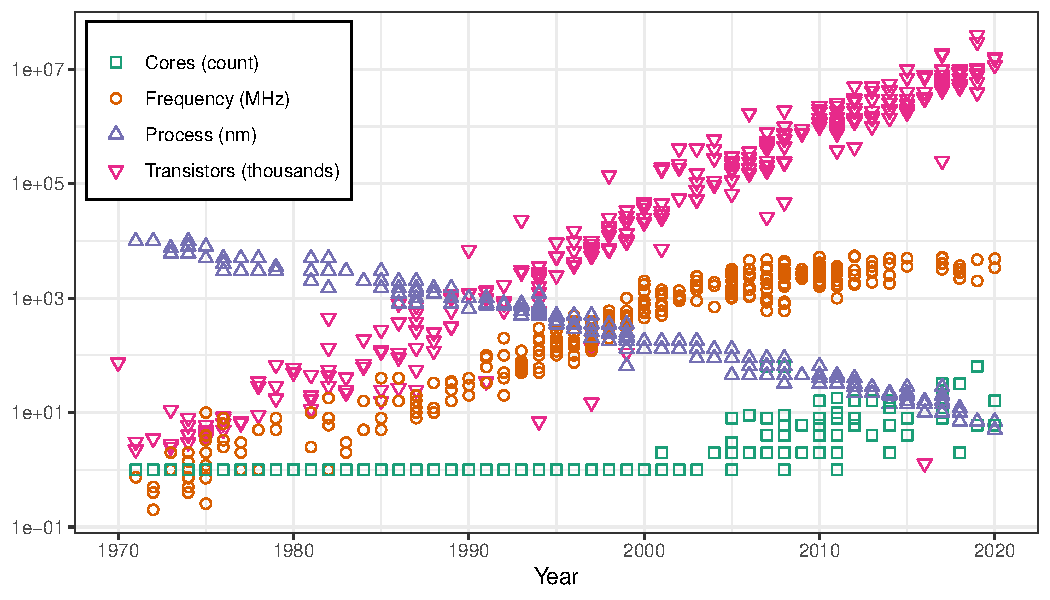
\includegraphics[width=\textwidth]{img/context/49_years.pdf}
            \caption{\label{fig:context:49_years}
            Evolution of the processor characteristics between 1971 and 2020. Plot inspired from the work of Pedro Bruel,
            generated with data from Wikipedia~\cite{wiki2021chronology,wiki2021transistor}.}
        \end{figure}

        One of the main contributions for this exponential growth of the number of transistors is the exponential
        decrease of their size, as plotted in Figure~\ref{fig:context:49_years}. While the IBM 608 calculator
        commercialized in the 50's had transistors ``no bigger than a paper clip''~\cite{ibm608}, the latest processors
        commercialized in 2020 have \NSI{5}{\nano\meter} transistors.

        In 1974, Dennard~\etal listed a set of rules for scaling silmutaneously the transistor density, clock frequency
        and power dissipation of processors~\cite{dennard}, which would eventually be named \emph{Dennard scaling}. The
        effect of this scaling on the device is summarized in Table~\ref{tab:dennard}. A scaling of \(\kappa\) will
        result in a clock frequency multiplied by a factor \(\kappa\) and a number of transistors multiplied by
        \(\kappa^2\) while the power density of the chip remains constant, \ie if the size of the processor does not
        change, it will have the same power consumption and generate the same amount of heat.

        \begin{table}[htpb]
            \centering
            \caption{Dennard scaling with a factor \(\kappa\) (table reproduced from~\cite[Table 1]{dennard}).}
            \label{tab:dennard}
            \begin{tabular}{l|c}
                Device or Circuit Parameter & Scaling Factor\\
                \hline
                Device dimension \(t_{ox}, L, W\) & \(1/\kappa\)\\
                Doping concentration \(N_a\) & \(\kappa\)\\
                Voltage \(V\) & \(1/\kappa\)\\
                Current \(I\) & \(1/\kappa\)\\
                Capacitance \(C=\epsilon A/t\) & \(1/\kappa\)\\
                Delay time/circuit \(VC/I\) & \(1/\kappa\)\\
                Power dissipation/circuit \(VI\) & \(1/\kappa^2\)\\
                Power density \(VI/A\) & 1\\
            \end{tabular}
        \end{table}

        Unfortunately, Dennard scaling came to an end 15 years ago. Indeed, it is no longer possible to scale the
        operating voltage and the gate oxide thickness~\cite{Bohr_2007}, as transistors have reached scales where power
        leakage is no longer negligible. With a voltage that cannot be scaled anymore, the power density cannot remain
        constant and reaches alarming levels of more than
        \NSI{4}{\watt/\milli\metre\squared}~\cite{Hennessy_2019,Hennessy_youtube}.

        \begin{figure}[htpb]
            \centering
            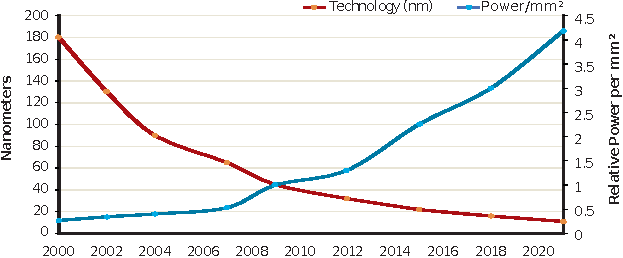
\includegraphics[width=\linewidth]{img/context/power_density.pdf}
            \caption{Evolution of the power density in the last 20 years (plot reproduced form ~\cite[Figure
            3]{Hennessy_2019}).}%
            \label{fig:context:power_density}
        \end{figure}

        Consequently, it has become impossible to increase further the CPU frequency, which has reached a limit of about
        \NSI{5}{\giga\hertz} since 2006 after an exponential growth of several decades, as shown by
        Figure~\ref{fig:context:49_years}. One of the response to keep the race for performance was to design multicore
        processors. Nowadays, nearly all laptops and smartphones have several cores, while high-end servers can have two
        or four sockets with up to 64 cores per socket.

        Yet, it appears that using several cores was only a short-term help for increasing the CPU
        performance. With the end of Dennard scaling, the power density increases with each generation of processor.
        Hence, to stay within a safe thermal design power (TDP), it is no longer possible to power at the nominal
        voltage all the components of the processors (notion named \emph{dark silicon}). Esmaeilzadeh~\etal predict
        that with the \NSI{8}{\nano\metre} processor generation, more than \NSI{50}{\percent} of their transistors might
        be unpowered at each given time~\cite{Esmaeilzadeh_2011}. With these constraints, Hennessy and
        Patterson~\cite{Hennessy_2019,Hennessy_youtube} estimate that the single-processor performance is now only
        growing by a mere \NSI{3}{\percent} per year, which is a much slower pace than the \NSI{50}{\percent} yearly
        growth rate that the industry got used to for decades.

        % First, performance gains are limited by Amdahl's law, stating that the maximal speedup obtained by running an
        % application on \(P\) cores is \(\frac{1}{(1-f) + f/P}\) where \(f\) is the fraction of the application that can
        % be run in parallel. For instance, an application whose \NSI{95}{\percent} of the execution can be made in
        % parallel will have a speedup of at most \(20\), even with an infinite number of cores.

    \section{Scientific computing today}%
    \label{sec:scientific_computing_today}

        \subsection{High performance computing}%
        \label{sub:hpc}

            Computations are now used in every scientific fields, from small statistical calculations to large numerical
            simulations. Science as a whole has immensely benefited from this exponential performance improvement. For
            instance, the price for sequencing an entire human genome has dropped from \SI{100000000}[\$]{} in 2001 to
            \SI{1000}[\$]{} in 2020~\cite{genome_sequencing}.

            To reach the highest performance, a single processor is not enough, the benefit of doing computations in
            parallel was already obvious at the time of human computers, as discussed in Section~\ref{sec:first_computers}.
            For this reason, the largest computations are now performed on supercomputers, large machines made of many
            processors connected through a fast network. The 500 fastest non-confidential supercomputers of the world are
            ranked biannually in the Top500~\cite{top500}. As shown by Figure~\ref{fig:context:top500}, they suffered from
            the same frequency staling as the rest of the industry in 2006, yet their performance kept an exponential
            increase, in part explained by the exponential increase of their total number of cores.

            \begin{figure}[htbp]
                \centering
                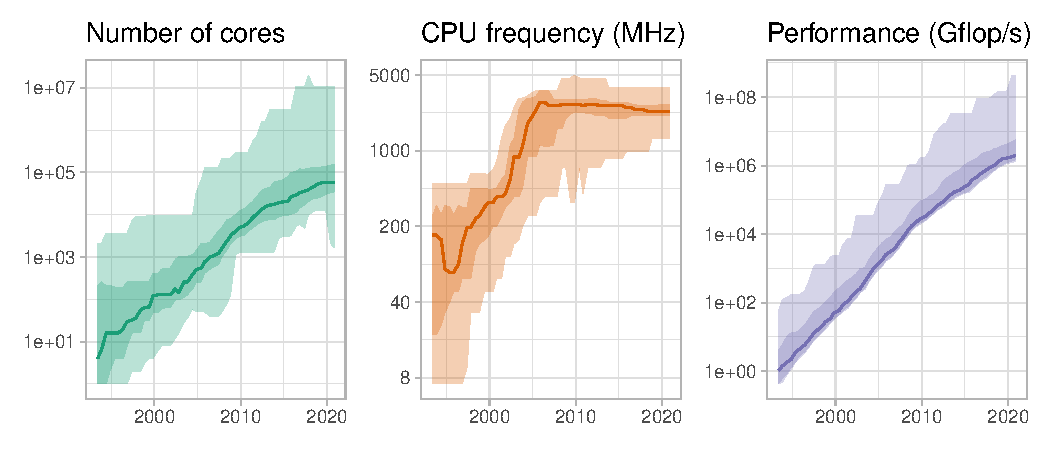
\includegraphics[width=\textwidth]{img/context/top500.pdf}
                \caption{\label{fig:context:top500}
                Evolution of the Top500~\cite{top500} supercomputers between 1993 and 2020.  The line denotes the median, the inner ribbon
                contains the \([\NSI{10}{\percent}, \NSI{90}{\percent}]\) interval, the outer ribbon contains all the
                values.\\ Data compiled by Dan Lenski~\cite{top500_compiled} and plotted by ourselves.}
            \end{figure}

            The largest supercomputers now have thousands of processors, millions of cores and power consumptions of several
            megawatts. At these scales, and with the hardware and software complexity required to reach the highest
            performance, it is extremely difficult to have an accurate picture of the whole platform. Even if all the
            individual components are deterministic at a microscopic level, a supercomputer observed at a macroscopic level
            can arguably be seen as a stochastic object. Hence, it is very common for the operators or the users of these
            machines to stumble on performance anomalies, \ie the \emph{observed} performance is different from the
            \emph{expected} performance. For instance, Petrini~\etal~\cite{Petrini_2003} found a severe but previously
            undetected performance problem on the supercomputer they were using, responsible of a \NSI{100}{\percent}
            performance variation and caused by operating system perturbations. Likewise,
            Tuncer~\etal~\cite[Section~1]{Tuncer_2017} list several examples of performance problems observed in operation:
            \begin{itemize}
                \item The amount of variation in application running time can reach \NSI{100}{\percent} on real-life
                    systems~\cite{Bhatele_2013,Skinner}.
                \item Orphan processes left over from previous jobs consumming system resources~\cite{Brandt_2010}.
                \item Firmware bugs, affecting the CPU usage on the server and making the user programs
                    fail~\cite{cisco_bug}.
                \item Memory leaks in applications, eventually leading to job failure~\cite{Agelastos_2015}.
                \item CPU throttling of the nodes for thermal control~\cite{Brandt2015EnablingAO}.
                \item Resource contention~\cite{Bhatele_2013,dorier:hal-00916091}.
            \end{itemize}
            If unnoticed, this kind of performance anomalies can affect very significantly the conclusions of an
            experimenter making performance measures on the machine.

        \subsection{A reproducibility crisis}%
        \label{sub:reproducibility_crisis}

            For several years there has been an ongoing concern of a reproducibility crisis in science. An online survey
            done in 2016 found that among the \Num{1576} scientists who responded, \NSI{70}{\percent} have failed at
            least once to reproduce the work of another scientist, \NSI{50}{\percent} have even failed to reproduce
            their own work~\cite{nature_survey}. This crisis is particularly concerning in medical science, where some
            researchers estimate that a large part of claimed research findings are
            false~\cite{Ioannidis_2005,freedman}. In this field, the main sources of non-reproducibility are a wrong
            usage of statistics, poor experimental methods or even frauds~\cite{science_misconduct}. In other
            disciplines such as computationnal biology or computationnal physics, reproducibility issues mainly come
            from numerical instability and the growing complexity of software environments~\cite{dong2021}.

            Computer science is not immune to these concerns of statistical misusage, numerical errors or frauds.  A
            recurrent problem is also the unavailability of the softwares, methods and data on which are based the
            research articles. For instance, Collberg~\etal examined 601 papers from ACM conferences and journals, they
            were able to personally build the software of only 194 of them while they simply could not access the code
            of 176 of these papers~\cite{collberg2015repeatability}. Likewise, Papadopoulos~\etal propose eight
            methodological principles for better reproducibility and show that most of the published articles
            they surveyed followed all these principles~\cite{Papadopoulos_2019}.

            What may be more surprising is that computer science suffers from the same experiment reproductibility
            problems than the other sciences, experimental biases exist and may even be larger. For instance,
            Mytkowicz~\etal show that simply changing the envifonment variable size can account for a performance
            variability of more than \NSI{30}{\percent}~\cite{Mytkowicz_2009}, they propose two methods for detecting
            and avoiding such measurement bias, based on experiment randomization. Similarly, Curtsinger and Berger have
            implemented a software for repeatedly re-randomizing the layouts of code, stack and heap at runtime, to
            avoid the bias introduced by a particular binary layout~\cite{stabilizer}. Again, the growing problem of
            experimental reproducibility we are describing here is tightly coupled to the growing software and hardware
            complexity.

    \section{This thesis}%
    \label{sec:this_thesis}

        In this thesis, we argue that a large part of computer science, and in particular high performance computing, is
        an experimental science. It is commonplace for computer scientists to run experiments, \eg for comparing the
        performance of several algorithms. With the kind of variability described in
        Section~\ref{sec:scientific_computing_today}, such experiments could easily lead to false conclusions. We
        therefore advocate for using similar methods to the natural sciences, which have been faced with the same issues
        for decades.

        Our contribution towards this goal of improving the confidence in the experimental results is multiple:
        \begin{itemize}
            \item In Part~\ref{part:prediction}, we propose a methodology for predicting the performance of an
                application through simulation. Similarly to biology or physics, making an experiment in simulation
                can be of great help to rule out part of the experimental bias. It can also enable the researchers to
                test scenarios that would be too costly in reality.
                \begin{itemize}
                    \item We contextualize this work in Chapters~\ref{chapter:prediction:related_work}
                        and~\ref{chapter:prediction:hpl}.
                    \item We explain how to improve the efficiency of the simulation in
                        Chapter~\ref{chapter:prediction:emulation}.
                    \item The models we used for the predictions are presented in
                        Chapter~\ref{chapter:prediction:modeling}.
                    \item Chapter~\ref{chapter:prediction:validation} is a thorough validation of the simulations, where
                        we compare the predicted performance with the observations made on real experiments.
                    \item We illustrate an important use case of such simulations in
                        Chapter~\ref{chapter:prediction:sensibility} by performing several sensibility studies.
                \end{itemize}
            \item In Part~\ref{part:experiment}, we present additional tools and methods to help experimenters increase
                the quality of their work.
                \begin{itemize}
                    \item Automation is a great way to improve both reliability and productivity. It helped tremendously
                        throughout the last century for scientific computations, as shown in
                        Section~\ref{sec:first_computers}, machines make much less mistakes than humans (if any) and
                        are much faster. For these reasons, we implemented several softwares during this thesis. We
                        automatized the execution of experiments with an experiment engine, presented in
                        Chapter~\ref{chapter:experiment:testbed}. We also implemented several tools, listed in
                        Chapter~\ref{chapter:zenodo}, for automating some parts of the analyses as well as cumbersome
                        daily tasks.
                    \item Several times during this thesis, our performance models were not in agreement with the
                        reality we observed. In some instances, our models were too simple and we needed to add
                        complexity to capture some real phenomena, as described in
                        Chapters~\ref{chapter:prediction:modeling} and~\ref{chapter:prediction:validation}. But, most of
                        the time, we suffered from an experimental bias (or the lack thereof). These difficulties are
                        described in depth in Chapter~\ref{chapter:experiment:difficulties}.
                    \item In an experimental work that span several years, like this thesis, it is very likely that the
                        experiment subject will evolve. In the case of high performance computing, the test machines can
                        have hardware or software upgrades, or even deffects, that can all affect significantly the
                        measured performance. In Chapter~\ref{chapter:experiment:tests}, we present the performance
                        non-regression tests we implemented and used in the second half of this thesis. They helped us
                        to detected numerous platform changes that could have lead to wrong conclusions if unnoticed.
                \end{itemize}
        \end{itemize}

        % \todo{
        % Performance anomalies $\rightarrow$ reproductibility problem (eg. if we compare two implementations, how can we be sure
        % that the difference we observe really come from the two implementations).
        % $\rightarrow$ Need a way for the users to have more confidence in their experiments.
        % $\rightarrow$ Several contributions towards this goal:
        % (1) Simulation of application, to remove the need of doing experiments.
        % (2) Automation of experiments (peanut), to reduce a lot the possibility of human mistakes.
        % (3) List several experimental difficulties, some of them very unsettling, to be aware of what can happen.
        % (4) Performance non regression tests of the platform, to detect significant changes.}

    % \section{Increased complexity}%
    % \label{sec:increased_complexity}

        % TODO increased complexity everywhere (HW and SW), deterministic at micro-level but the macro-level is random
        % no complete understanding of the whole thing, we need experimental CS, we need models (very similarly to what
        % is done in physics or biology)
    %     Some horror stories~\cite{Petrini_2003}\dots
